\begin{ZhChapter}

\chapter{研究方法}

\section{}

在傳統軟體開發生命週期中,系統測試(System Testing)負責驗證完全整合後的產品是否符合規格要求,是品質保證(Quality Assurance, QA)對照初期需求進行全面驗收的重要階段。然而,隨著對開發速度與彈性的需求不斷提升,特別是在敏捷(Agile)方法興起後,耗時且成本高昂的測試流程(例如大規模回歸測試)逐漸被視為難以持續。組織投入於品質保證與測試的資源已占據 IT 預算的相當比例,使得過去將測試視為獨立階段的做法難以因應當前需求。
因此,系統測試逐漸從傳統的後置活動,轉變為嵌入短週期開發衝刺(Sprint)中的持續性驗證與確認(Continuous V&V)流程。這一轉變促使「自動化測試」(Automated Testing)在軟體開發中迅速普及,QA 團隊開始撰寫可重複執行的測試腳本,以確保功能在頻繁修改下仍保持正確性。
隨著 CI/CD 的導入,快速部署與「持續測試」(Continuous Testing)成為現代 DevOps 實踐的核心,用以縮短從程式碼提交到上線的整體時間。自動化的系統測試與整合測試被內嵌於 CI/CD 管線(Pipeline)中,使其成為穩定交付品質的必要條件。\cite{TestingSoftwareSystems}
\begin{itemize}
    \item 持續整合(CI):開發者頻繁將程式碼合併至中央倉儲,每次合併都會自動觸發建構(Build)及自動化測試(通常涵蓋單元測試及整合測試)。
    \item 持續部署(CD):作為 CI 的延伸,當程式碼通過所有自動化測試後,可自動部署至預備環境或生產環境。
\end{itemize}

為實現上述目標,本研究提出之「自主測試與文件生成框架 (V-Final)」如下圖 1-1 所示。
\begin{figure*}[htbp]
    \centering
    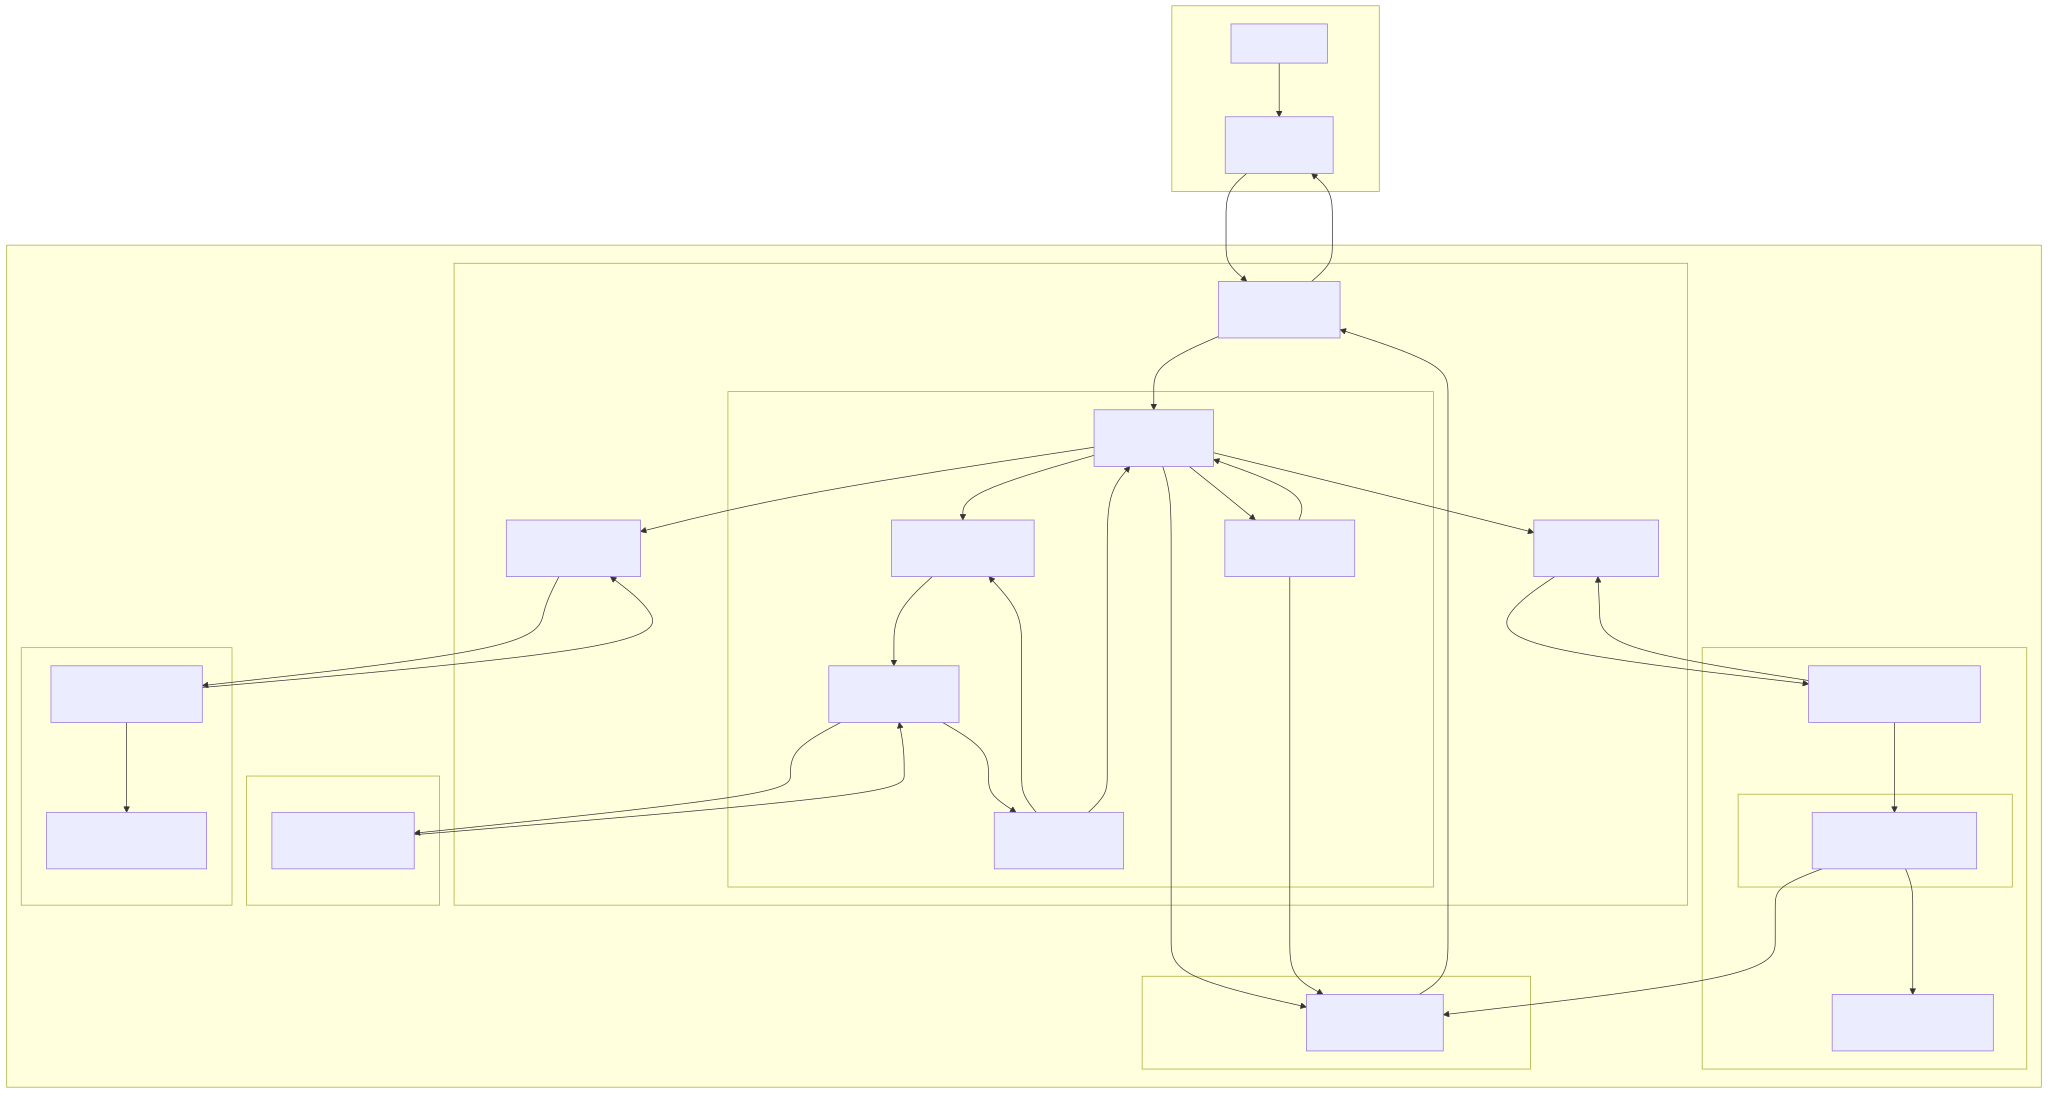
\includegraphics[width = 1.0\textwidth]{static-page/architecture.png}
    \caption{Cool train station}
    \label{fig: image}
\end{figure*}

% \begin{table*}[htbp]
%     \centering
%     \caption{表格範例標題} \label{tab: complexity}
%     \makebox[\linewidth][c]{
%     \renewcommand\arraystretch{1.2}{
%         \begin{tabular}{| l | c  c  c  c |}
%         \hline
%         Protocol & $P$ & $CS_1$ & $CS_2$ & $RG$ \\
%         \hline
%         MSSMul & $O(1)$, $O(1)$, N/A & $O(n-t)$, $O(n)$, $O(1)$ & $O(n-t)$, $O(n)$, N/A & $O(1)$, $O(n)$, $O(n)$ \\
%         SC & $O(1)$, $O(1)$, N/A & $O(n-t)$, $O(n)$, $O(1)$ & $O(n-t)$, $O(n)$, N/A & $O(1)$, $O(n)$, $O(n)$ \\
%         \hline 
%         \end {tabular}
%     }}
% \end {table*}

% \section{模型說明(小標)}

% 說明說明說明說明,說明說明說明說明說明說明說明說明說明說明說明說明,說明說明說明說明說明說明說明說明。

% \begin{figure*}[htbp]
%     \centering
%     \includegraphics[width = 0.5\textwidth]{image.jpeg}
%     \caption{Cool train station}
%     \label{fig: image}
% \end{figure*}

\end{ZhChapter}